%%%%%%%%%%%%%%%%%%%%%%%%%%%%%%%%%%%%%%%%%
% Short Sectioned Assignment
% LaTeX Template
% Version 1.0 (5/5/12)
%
% This template has been downloaded from:
% http://www.LaTeXTemplates.com
%
% Original author:
% Frits Wenneker (http://www.howtotex.com)
%
% License:
% CC BY-NC-SA 3.0 (http://creativecommons.org/licenses/by-nc-sa/3.0/)
%
%%%%%%%%%%%%%%%%%%%%%%%%%%%%%%%%%%%%%%%%%

%----------------------------------------------------------------------------------------
%	PACKAGES AND OTHER DOCUMENT CONFIGURATIONS
%----------------------------------------------------------------------------------------

\documentclass[paper=a4, fontsize=11pt]{scrartcl} % A4 paper and 11pt font size

\usepackage[T1]{fontenc} % Use 8-bit encoding that has 256 glyphs
\usepackage{fourier} % Use the Adobe Utopia font for the document - comment this line to return to the LaTeX default
\usepackage[english]{babel} % English language/hyphenation
\usepackage{amsmath,amsfonts,amsthm} % Math packages

\usepackage{lipsum} % Used for inserting dummy 'Lorem ipsum' text into the template

\usepackage{sectsty} % Allows customizing section commands
\allsectionsfont{\normalfont\scshape} % Make all sections centered, the default font and small caps
\usepackage{graphicx}
\usepackage{float}
\usepackage{fancyhdr} % Custom headers and footers
\pagestyle{fancyplain} % Makes all pages in the document conform to the custom headers and footers
\fancyhead{} % No page header - if you want one, create it in the same way as the footers below
\fancyfoot[L]{} % Empty left footer
\fancyfoot[C]{} % Empty center footer
\fancyfoot[R]{\thepage} % Page numbering for right footer
\renewcommand{\headrulewidth}{0pt} % Remove header underlines
\renewcommand{\footrulewidth}{0pt} % Remove footer underlines
\setlength{\headheight}{13.6pt} % Customize the height of the header

\numberwithin{equation}{section} % Number equations within sections (i.e. 1.1, 1.2, 2.1, 2.2 instead of 1, 2, 3, 4)
\numberwithin{figure}{section} % Number figures within sections (i.e. 1.1, 1.2, 2.1, 2.2 instead of 1, 2, 3, 4)
\numberwithin{table}{section} % Number tables within sections (i.e. 1.1, 1.2, 2.1, 2.2 instead of 1, 2, 3, 4)

\setlength\parindent{0pt} % Removes all indentation from paragraphs - comment this line for an assignment with lots of text

%----------------------------------------------------------------------------------------
%	TITLE SECTION
%----------------------------------------------------------------------------------------

\newcommand{\horrule}[1]{\rule{\linewidth}{#1}} % Create horizontal rule command with 1 argument of height

\title{	
\normalfont \normalsize 
\textsc{CS 287 - John A. Paulson School of Engineering and Applied Sciences} \\ [25pt] % Your university, school and/or department name(s)
\horrule{0.5pt} \\[0.4cm] % Thin top horizontal rule
\huge Project Update - Memory Networks For Question Answering \\ % The assignment title
\horrule{2pt} \\[0.5cm] % Thick bottom horizontal rule
}

\author{Nicolas Drizard \& Virgile Audi\\
nicolas.drizard@g.harvard.edu\quad vaudi@g.harvard.edu} % Your name

\date{\normalsize\today} % Today's date or a custom date

\begin{document}

\maketitle % Print the title

%----------------------------------------------------------------------------------------
% Introduciton %----------------------------------------------------------------------------------------

\section*{Introduction}

The focus of this final project is about non-factoid question answering. To tackle this problem, we chose to implement memory network type of models and in particular the dynamic memory network presented in \cite{dmn}. For this project update, we mainly worked on pre-processing the data from the bAbi dataset, implementing a count-base baseline as well as looking at a one hop memory weakly supervised memory network.


%------------------------------------------------

\section{Data Pre-processing}

Our goal is to build a robust model, i.e. working on any kind of task of question answering. The bAbI dataset created by Facebook \cite{aiqua} provides us relevant tasks. We ore-processed it in several steps:

First, we mapped each word to an index. We know that every answer word from the test set is used as anwser in the test set, so this index is built only on the train set but used for both train and test set.

Second, we pre-process each sentence as a bag og words, i.e. we convert it to a vector of word indexes of fixed length (the maximum length over the sentences), using a padding index of 0 at the end. We separate in two different array the sentences and the questions, both are indexed globally in the given dataset.

Third, we encoded in one array the links between the questions and the sentences. Each row corresponds to the question with the corresponding global index in the dataset and contains: index of the first and last sentences of the story and the indexes of its supporting facts. This later is a fixed size list, with a 0 padding for question with less supporting facts.

Finally, we store in one vector the word index of the answer for each question. This matrix may have multiple columns with a 0 padding if some questions contain several answers.


\section*{Baseline}
As a baseline, we decided to apply a count based approach. We developped two main features and also tried to introduce a first step to narrow the story to only the relevant facts given the question

\subsection*{Count Based Model}
\paragraph{Answer words counts in the story}
The first feature evaluate the presence of each answer word in the story, weighted with a decay depending on when it occurs in the story. The idea is basically to count the decayed occurrences of each possible answer word in the story and then to normalize it. It's a simple function taking as input a story, i.e. sequence of facts seen as a bag of words, and return a distribution over the possible answer words. (We know that all the answer words in the test questions have been answer word in the train).


We use a simple affine function for the decay with a smoothing parameter $\alpha_1$ to be more resilient:
\[
\tilde{f}_1(x_i) = \alpha_1 \sum_k^{|AW|}\delta_1(x_i = aw_k)(1 + \beta * i)
\]
with $x_i$ the word of index i in the story, $AW$ the set of possible answer words and $\delta_1(x_i = aw_k)$ a one hot vector of size $|AW|$ with a one on the $k^{th}$ if $x_i = aw_k$. We used in the experiments: $\alpha_1 = 0.1$ and $\beta = 0.15$.


For a given story $X=(x_1, ..., x_S)$, we have the corresponding $f_1$ feature:

\[
f_1(X) = \sum_{i=1}^S\tilde{f}_1(x_i)
\]

This feature is easy to build for a baseline but contains a lot of drawbacks. First, we just apply a dummy decay over the time. For instance if the answer of a question relies in the first sentence of a story and then comes several sentences without any extra information relative to the question but with possible answer words these wil get a higher score than the real answer. Furthermore, we are not using the question in this feature. Moreover, this feature is just extracted on the fly from the input and we don't take advantage of the train test we have. 

\paragraph{Question embeddings}

This feature aims to use the question, especially the kind of answers it expects: yes/no question, locations, activity, person... This information relies mainly in the question word. As a result, we just extract the first word of the question and embedd it as a vector of size $|AW|$. This embedding is learned at train time and corresponds to the occurences of each answer words as answer to a question with this specific answer words (with a smoothing $\alpha_2$). It will provide a prior information on the expected answer given the question word.

For a given question $Q = (q_1, ..., q_{|Q|}))$:

\[
f_2(Q) = \tilde{f}_2(q_1) = \alpha_2 + \sum_{i = 1}^{N_{train}} \mathbb{1}(q_1^{(i)}=q_1) \delta_2(q_1, aw_i)
\]

with $q_1^{(i)}$ the first word of the $i_{th}$ question fromt the train set and $\delta_2(aw_i)$ a one hot vector of size $|AW|$ with a one on the $i^{th}$ . We use in the experiments $\alpha_2 = 0.1$ 

This feature takes advantage of the train set and uses part of a question on contrary to the first feature. We could still extend it while using the rest of the question also. 

\paragraph{Prediction}

The input of the model is a tuple story, question $(X,Q)$. We treat the feature as independant probability distribution as in the Naive Bayes approach so we just simply combine the feature witha product. In the experiment we treat them in the log space for computational purpose and take the argmax of the vector coordinates

Concretely

\[
\hat{y}(X,Q) = argmax(\log(f_1(X)) + \log(f_2(Q)))
\]


\paragraph{Sentence Matching}

Here, we introduce a preliminary step to restrict the number of sentences of a given story given the question, i.e. looking for the supporing facts. A first idea, inspired by \cite{mct}, is to use occurences of words in the questions in the story. We can then decide to output one of several supporting facts.

Moreover,if we consider the following example:\\
\begin{center}
Mary picked up the football.\\
Mary went to the garden.\\
John walked to the garden.\\
Where is the football?
\end{center}

Here, simple occurences are not enough. We need to look for sentences that have other co-occurences with the sentences that scored in the first question/sentence matching. The word "Mary" then enables to return the relevant facts to answer the question.\\

One drawback is on the returned number of supporting facts. The maximum number should be less than three as in the data set but more sentence may match. Nevertheless, this step would only be necessary for the count-base model. And since the use of this model was just to act as a baseline to the memory networks, we decided that the model performed sufficiently well to leave it to that.

\subsection{Results}

We applied the two models on the train and test set, the feature $f_1$ is computed on the fly and $f_2$ was learned on the train set. We obtained fairly good results, even better than those provided in \cite{aiqua} on average. We provided the size of the output space $|AW|$ for each question to have an idea of a model with random guess. But we trained all the tasks globaly, ie with an output vector in the global output space. We are not able to provide results on tasks 8 and 19 as they expect outputs with different sizes (List and Path finding). We chose not to focus on these ones but will try to adapt our memory network to them.

For instance, it seems to provide acceptable results on the first three tasks, as usually the answer appears always at the end of the story; or at least it's the last word in the set of expected words given the question word. (For instance last location words for a \textit{Where}). On the contrary, on Yes/no tasks (6, 17, 18) the results are almost random (around 50\% of accuracy) as the answer Yes/no do not appear in the story.

\begin{figure}[H]
\centering
\begin{minipage}{.5\textwidth}
\centering
\caption{Results on TRAIN}
\label{my-label}
\begin{tabular}{|l|l|l|}
\hline
Task & \ |AW| & Accuracy \\ \hline
1    & 6                   & 54       \\ \hline
2    & 6                   & 38       \\ \hline
3    & 6                   & 29       \\ \hline
4    & 6                   & 33       \\ \hline
5    & 7                   & 54       \\ \hline
6    & 2                   & 49       \\ \hline
7    & 4                   & 49       \\ \hline
8    & -                   & 0        \\ \hline
9    & 2                   & 63       \\ \hline
10   & 3                   & 47       \\ \hline
11   & 6                   & 62       \\ \hline
12   & 6                   & 58       \\ \hline
13   & 6                   & 71       \\ \hline
14   & 6                   & 28       \\ \hline
15   & 4                   & 16       \\ \hline
16   & 4                   & 51       \\ \hline
17   & 2                   & 50       \\ \hline
18   & 2                   & 50       \\ \hline
19   & 4                   & 0        \\ \hline
20   & 7                   & 56       \\ \hline
\end{tabular}
\end{minipage}%
\begin{minipage}{.5\textwidth}
\centering
\caption{Results on TEST}
\label{my-label}
\begin{tabular}{|l|l|l|}
\hline
Task & |AW| & Accuracy \\ \hline
1    & 6                   & 50       \\ \hline
2    & 6                   & 40       \\ \hline
3    & 6                   & 26       \\ \hline
4    & 6                   & 34       \\ \hline
5    & 7                   & 48       \\ \hline
6    & 2                   & 50       \\ \hline
7    & 4                   & 49       \\ \hline
8    & -                   & 0        \\ \hline
9    & 2                   & 64       \\ \hline
10   & 3                   & 44       \\ \hline
11   & 6                   & 63       \\ \hline
12   & 6                   & 60       \\ \hline
13   & 6                   & 68       \\ \hline
14   & 6                   & 29       \\ \hline
15   & 4                   & 14       \\ \hline
16   & 4                   & 52       \\ \hline
17   & 2                   & 48       \\ \hline
18   & 2                   & 53       \\ \hline
19   & 4                   & 0        \\ \hline
20   & 7                   & 52       \\ \hline
\end{tabular}
\end{minipage}
\end{figure}

\section{Memory Network}

If we didn't have sufficient time to implement a first memory network, we wanted to present the first memory network we will implement. The model was introduced in \cite{mem} and can be summarised in the following graphical representation:

\begin{figure}[H]
\begin{center}
    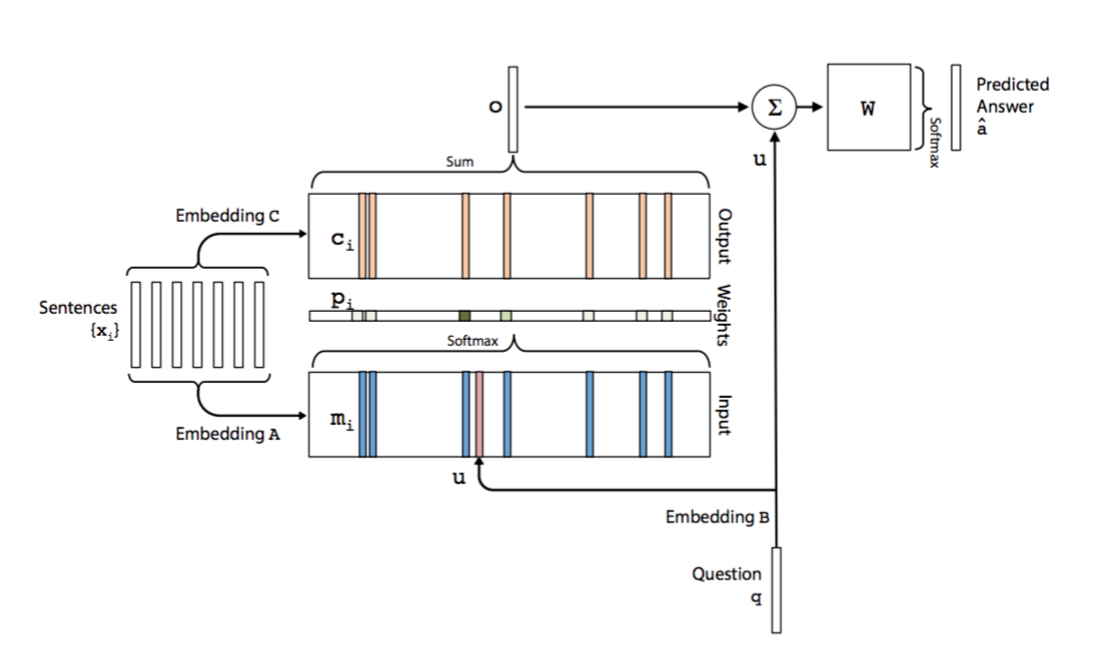
\includegraphics[width=0.7\textwidth]{mem.png}
    \caption{1-Hop Memory Network}
\end{center}
\end{figure}

This model implements a single memory hop operation. This model takes for inputs the question and the sentences of the story. The sentences of the story are then embedded with two differents look-up tables. The first look-up table (which corresponds to the matrix A in the above diagram) will be used to store the sentences of the stories as input in memory. These embedded representation of the story's sentences will then be combined with the embedded representation of the question (using the matrix B) using a dot product. The result of this dot product is then passed through a softmax layer to give a probability distribution over which sentence is likely to give information about the answer. The memory output vector $o$ results from a weighted sum of the output embeddings of the sentences (using matrix C) using the probability distribution $p$. We then apply a weight matrix to the sum of question embeddings and the output vector $o$ followed by a softmax to predict the answer. We can summarize this process with the formula:

$$\hat{a} = \text{softmax}\left(W(o+u)\right)$$
where: $ o = \sum\limits_{i=1}\text{softmax}(u^Tm_i)$, with $u$ being the embedded representation of the question and $m_i$ the embedded represenation of the sentence $i$ in the story.\\

The embedded representation of sentences and questions can either be obtained by summing the embeddings of their words or by concatenating them. We plan on testing the two approaches.\\

Finally, we will implement a temporallity feature by modifying the embedded representation of the sentences by adding a term depending on the index of the sentence in the story.

\section{Future Steps}

If we plan to code this model using the regular "nn" module, we would also like to use the "nngraph" module. Indeed, once this model implemented, we would like to implement a variation by adding mutliple hops to memory. This model is also presented in \cite{mem} and its structure could be too complex for the "nn" module. We will then tackle the dynamic memory network that we introduced in the proposal and can be found in \cite{dmn}.
%----------------------------------------------------------------------------------------
\bibliographystyle{apalike}
\bibliography{update}
\end{document}